% @Author: AnthonyKenny98
% @Date:   2020-02-27 14:22:10
% @Last Modified by:   AnthonyKenny98
% @Last Modified time: 2020-04-06 15:16:33

\begin{figure}[H]
\begin{center}
\begin{tabular}{c c}

    % Subfigure A
    \begin{subfigure}{0.45\textwidth}
    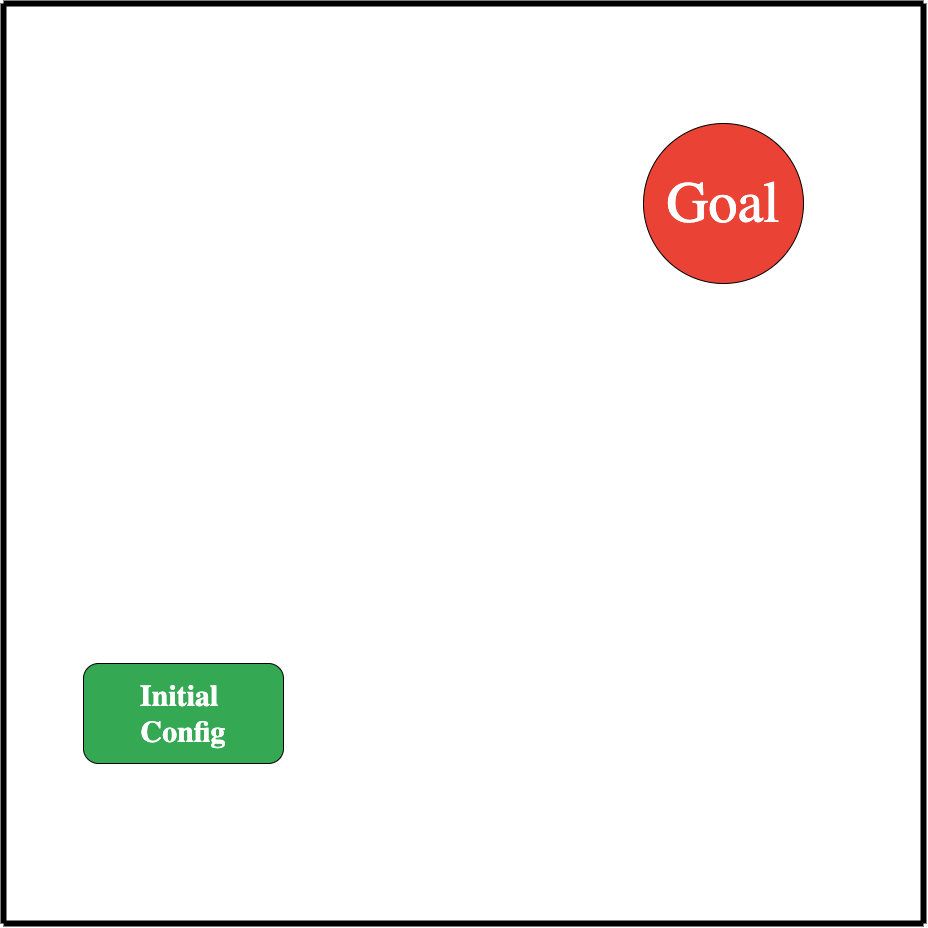
\includegraphics[width=\linewidth]{chapters/chapter2/img/RRT_step_by_step-A.png}
    \caption{}
    \label{subfig:rrt-step-by-step-A}
    \end{subfigure} &
    % 
    % Subfigure B
    \begin{subfigure}{0.45\textwidth}
    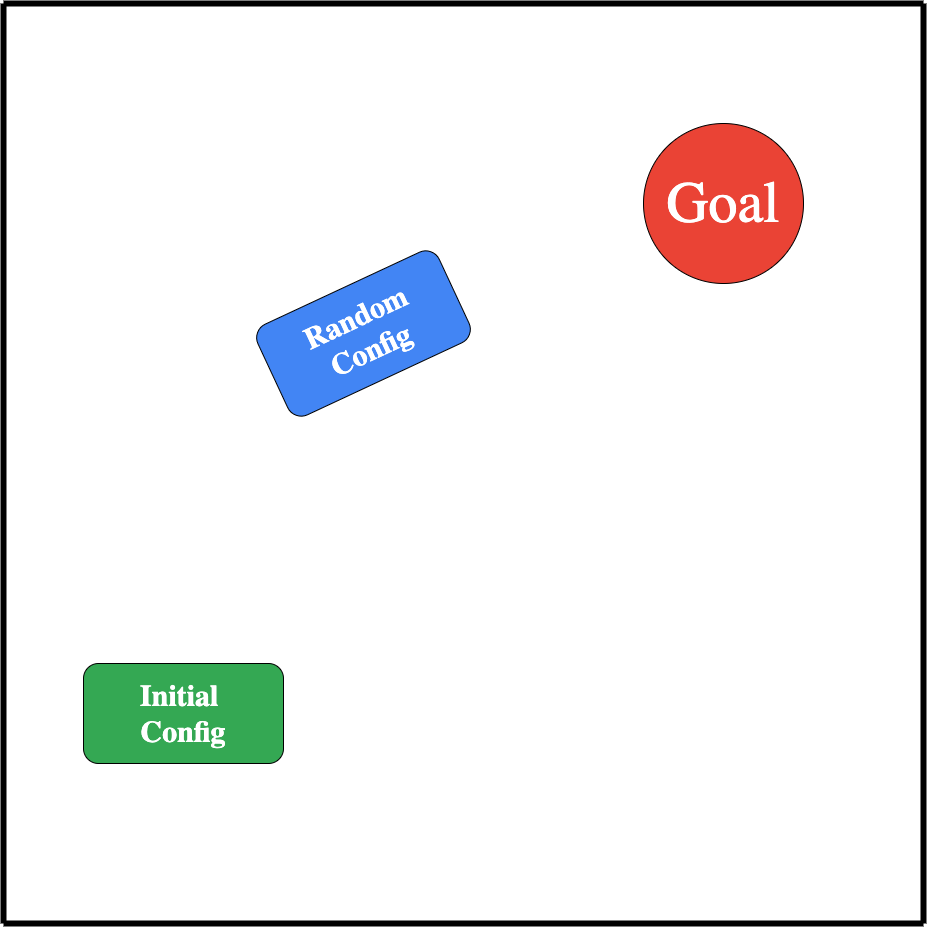
\includegraphics[width=\linewidth]{chapters/chapter2/img/RRT_step_by_step-B.png}
    \caption{}
    \label{subfig:rrt-step-by-step-B}
    \end{subfigure} \\

    % Subfigure C
    \begin{subfigure}{0.45\textwidth}
    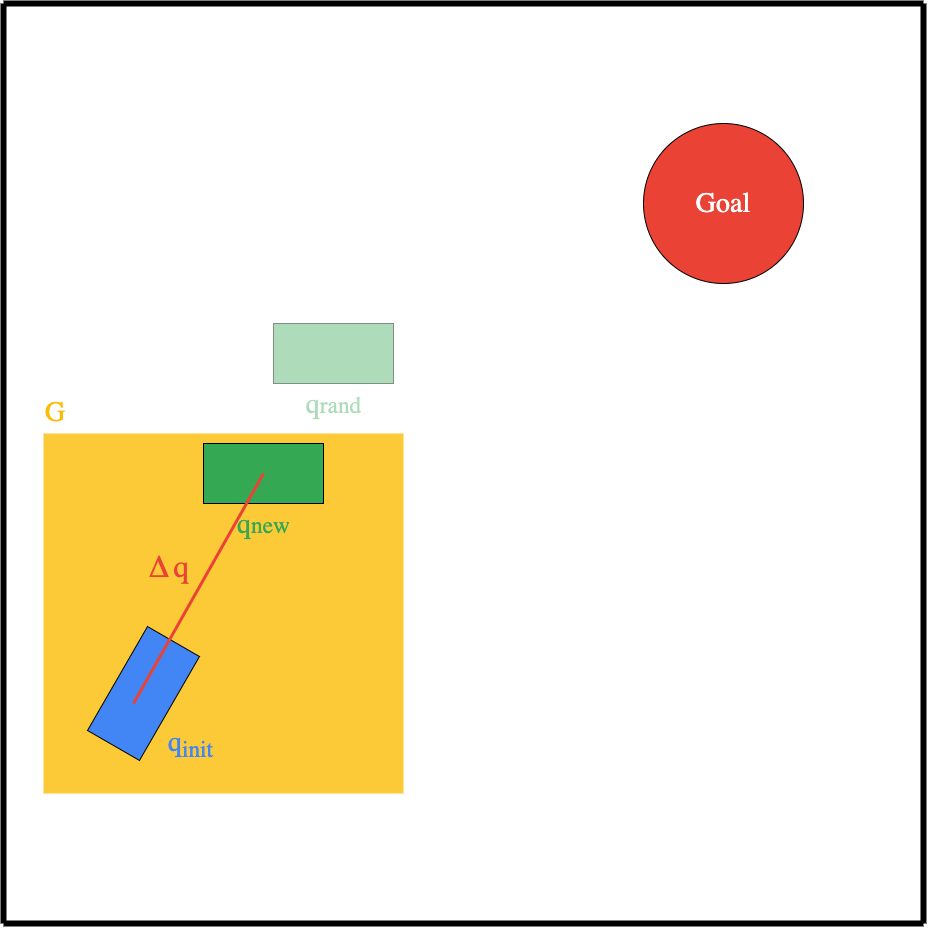
\includegraphics[width=\linewidth]{chapters/chapter2/img/RRT_step_by_step-C.png}
    \caption{}
    \label{subfig:rrt-step-by-step-C}
    \end{subfigure} &
    % 
    % Subfigure D
    \begin{subfigure}{0.45\textwidth}
    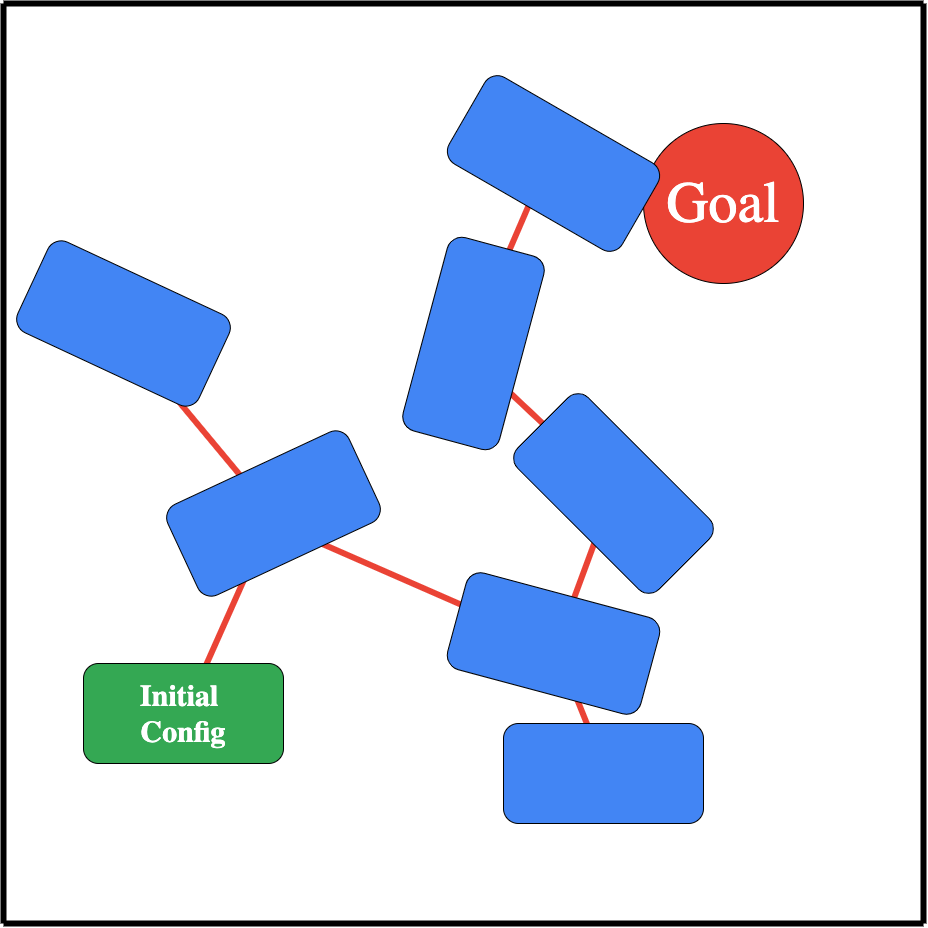
\includegraphics[width=\linewidth]{chapters/chapter2/img/RRT_step_by_step-D.png}
    \caption{}
    \label{subfig:rrt-step-by-step-D}
    \end{subfigure}

\end{tabular}
    
    % Caption and Label
    \mycaption{Demonstration of \gls{RRT} Algorithm for 2D robot in 2D space.}{ In this example, the graph $G$ begins with an initial configuration and a goal. In (b), the first random configuration is generated. In this case, the nearest configuration is the inital configuration. The random configuration is more than $\epsilon$ from the initial configuration, so a new configuration in the direction of the random configuration is generated and added to the graph in (c). This is repeated $K$ times, until the graph in (d) is generated.}
    \label{fig:rrt-step-by-step}
\end{center}
\end{figure}